\section{Pendahuluan}
\subsection{Latar Belakang}
Seiring dengan berkembangnya teknologi digital, jaringan komputer menjadi komponen krusial dalam mendukung komunikasi dan pertukaran informasi antarsistem secara efisien. Meskipun kini telah tersedia IPv6, protokol IPv4 masih mendominasi dalam penerapan jaringan di berbagai sektor. Oleh karena itu, pemahaman mendalam tentang jaringan berbasis IPv4 merupakan keterampilan dasar yang wajib dimiliki oleh para profesional di bidang teknologi informasi. Permasalahan yang sering dijumpai di lapangan meliputi konflik IP address, pemisahan subnet yang tidak tepat, hingga kendala komunikasi antarperangkat. Praktikum ini memberikan pengalaman langsung kepada mahasiswa dalam membangun dan mengelola jaringan, dimulai dari pembuatan kabel (crimping) hingga konfigurasi routing baik secara manual maupun otomatis. Materi ini penting karena banyak diterapkan dalam lingkungan akademik, lembaga pemerintahan, hingga perusahaan, sehingga penguasaan konsep-konsep jaringan akan memperkuat kesiapan mahasiswa dalam dunia kerja.

\subsection{Dasar Teori}
Dalam jaringan komputer, sambungan fisik antarperangkat merupakan fondasi utama sebelum konektivitas logis dapat dijalankan. Salah satu komponen penting dalam tahapan ini adalah proses crimping, yakni teknik pemasangan konektor RJ-45 ke ujung kabel UTP menggunakan alat khusus bernama crimping tool. Kabel UTP terdiri dari delapan kawat tembaga yang dibungkus berpasangan, dan susunan kabelnya harus mengikuti standar internasional seperti T568A atau T568B. Penyusunan urutan kabel yang tepat sangat menentukan kestabilan jaringan; kesalahan kecil dalam proses ini dapat menyebabkan sinyal terganggu, koneksi tidak terbaca, atau bahkan kehilangan data. Oleh karena itu, presisi dalam proses crimping menjadi hal yang sangat krusial dalam membangun infrastruktur jaringan yang andal.

Setelah perangkat terhubung secara fisik, pengaturan jalur komunikasi antarjaringan dilakukan melalui proses routing. Routing pada jaringan berbasis IPv4 bertujuan mengarahkan paket data dari satu alamat IP ke alamat tujuan melalui jalur yang paling efisien. Setiap perangkat dalam jaringan memiliki alamat IP unik untuk identifikasi, dan router bertugas memilih jalur data berdasarkan konfigurasi yang telah ditentukan. Ada dua pendekatan umum dalam routing: secara manual melalui konfigurasi statis yang tetap, dan secara otomatis melalui protokol dinamis seperti RIP, OSPF, atau EIGRP yang mampu menyesuaikan jalur berdasarkan perubahan kondisi jaringan. Routing ini melibatkan konsep seperti jumlah lompatan (hop count), tabel routing, dan pemilihan jalur optimal untuk memastikan komunikasi antarjaringan berjalan lancar, cepat, dan handal.

%===========================================================%
\section{Tugas Pendahuluan}
	\subsection*{1. Perencanaan Alokasi IP Address dan CIDR}
Perancangan jaringan dilakukan menggunakan alamat privat \texttt{192.168.0.0/24} dengan metode VLSM untuk efisiensi. Alokasi subnet sebagai berikut:

    \textbf{Departemen R\&D} (100 perangkat): \texttt{192.168.0.0/25} \\
    Rentang host: \texttt{192.168.0.1 – 192.168.0.126}, Broadcast: \texttt{192.168.0.127}

    \textbf{Departemen Produksi} (50 perangkat): \texttt{192.168.0.128/26} \\
    Rentang host: \texttt{192.168.0.129 – 192.168.0.190}, Broadcast: \texttt{192.168.0.191}

    \textbf{Departemen Administrasi} (20 perangkat): \texttt{192.168.0.192/27} \\
    Rentang host: \texttt{192.168.0.193 – 192.168.0.222}, Broadcast: \texttt{192.168.0.223}
    
    \textbf{Departemen Keuangan} (10 perangkat): \texttt{192.168.0.224/28} \\
    Rentang host: \texttt{192.168.0.225 – 192.168.0.238}, Broadcast: \texttt{192.168.0.239}

Total terdapat 4 subnet yang efisien dan tidak saling tumpang tindih.

	\subsection*{2. Topologi Jaringan}

Topologi menggunakan satu router utama yang menghubungkan masing-masing departemen melalui port berbeda atau VLAN terpisah. Setiap subnet dihubungkan ke router melalui interface khusus:

\begin{center}
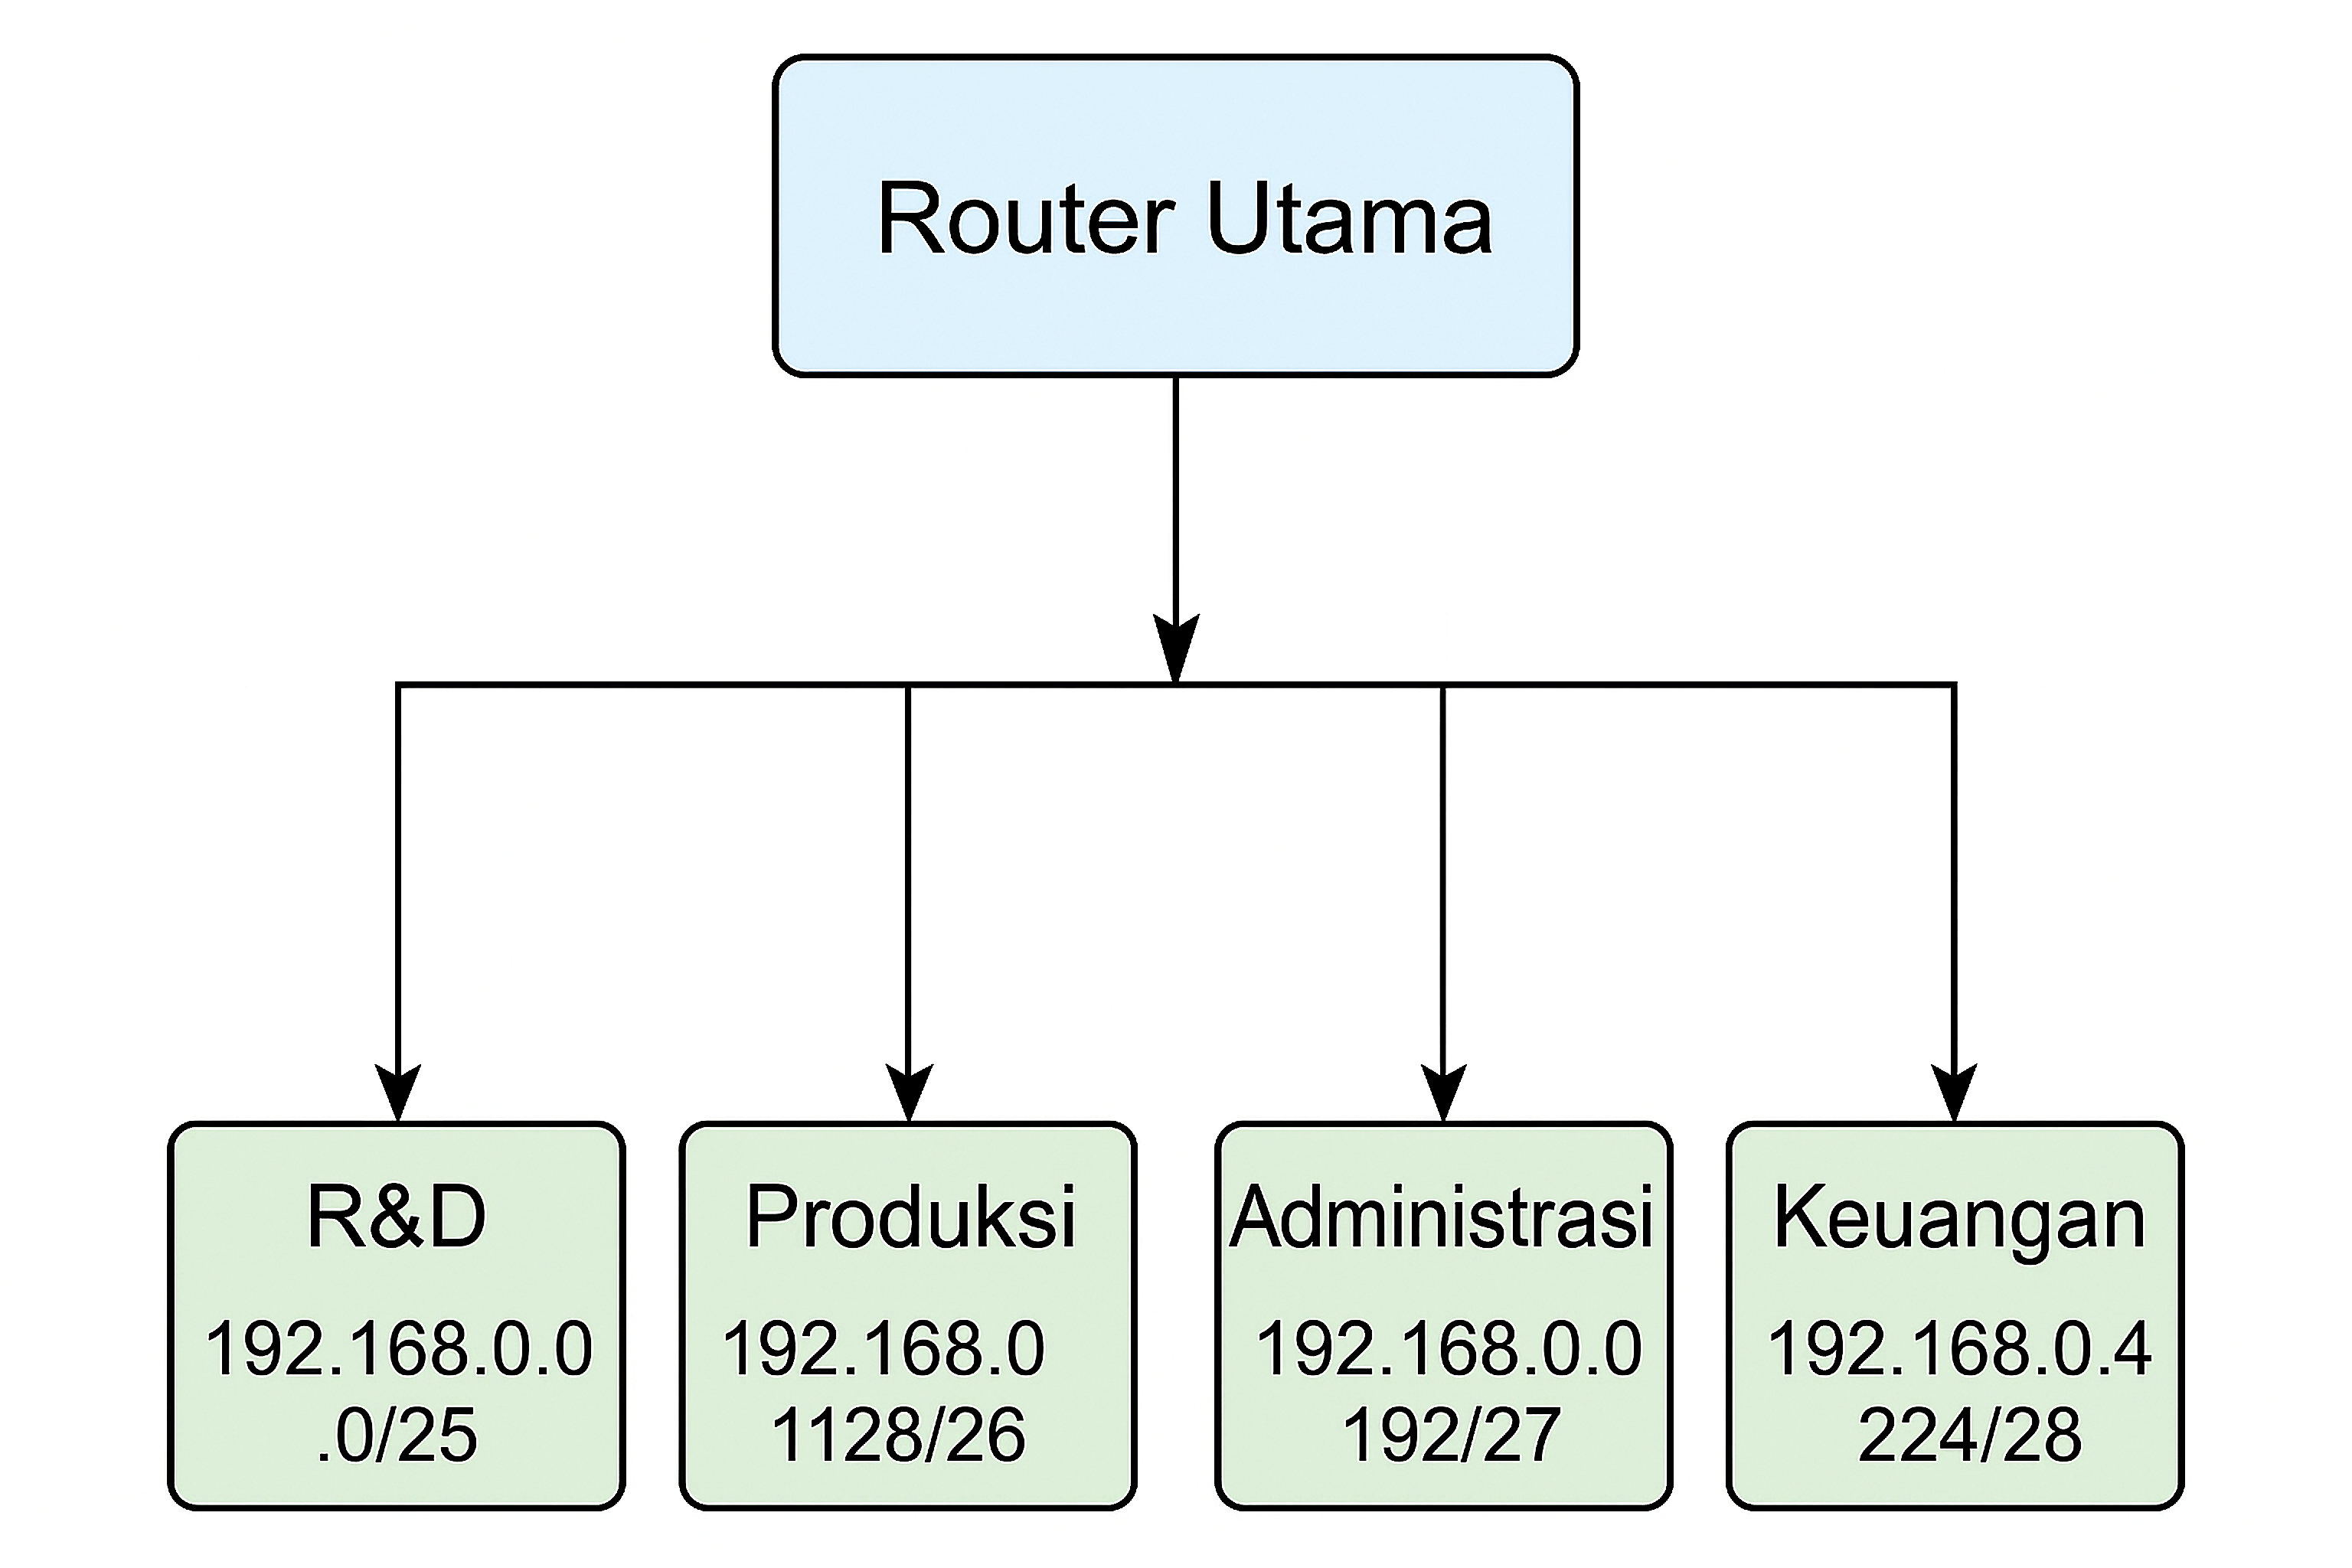
\includegraphics[width=0.8\textwidth]{P1/img/topologi.png}
\end{center}

	\subsection*{3. Tabel Routing}

\begin{tabular}{|l|l|l|}
\hline
\textbf{Network} & \textbf{Prefix} & \textbf{Interface Router} \\
\hline
192.168.0.0 & /25 & Gig0/0 (R\&D) \\
192.168.0.128 & /26 & Gig0/1 (Produksi) \\
192.168.0.192 & /27 & Gig0/2 (Administrasi) \\
192.168.0.224 & /28 & Gig0/3 (Keuangan) \\
\hline
\end{tabular}

        \subsection*{4. Jenis Routing yang Digunakan}

Jenis routing yang digunakan adalah \textbf{Static Routing}, karena sifat jaringan yang sederhana dan stabil. Dengan hanya satu router dan empat subnet tetap, tidak diperlukan mekanisme pertukaran informasi routing secara dinamis. Keuntungan lainnya adalah efisiensi penggunaan sumber daya perangkat keras dan kemudahan dalam konfigurasi serta pemeliharaan.

Namun, jika di masa depan terjadi ekspansi jaringan, misalnya penambahan cabang atau subnet baru, maka protokol routing dinamis seperti OSPF dapat dijadikan alternatif karena mendukung skala besar serta fleksibel terhadap perubahan. Dalam desain ini, prinsip CIDR telah diterapkan agar alokasi IP tetap optimal dan mudah diatur.